\chapter{The Program}
\label{app:A}

The interface of the program is shown in Figure~\ref{fig:appxa2}:

\begin{figure}[H]
\centering
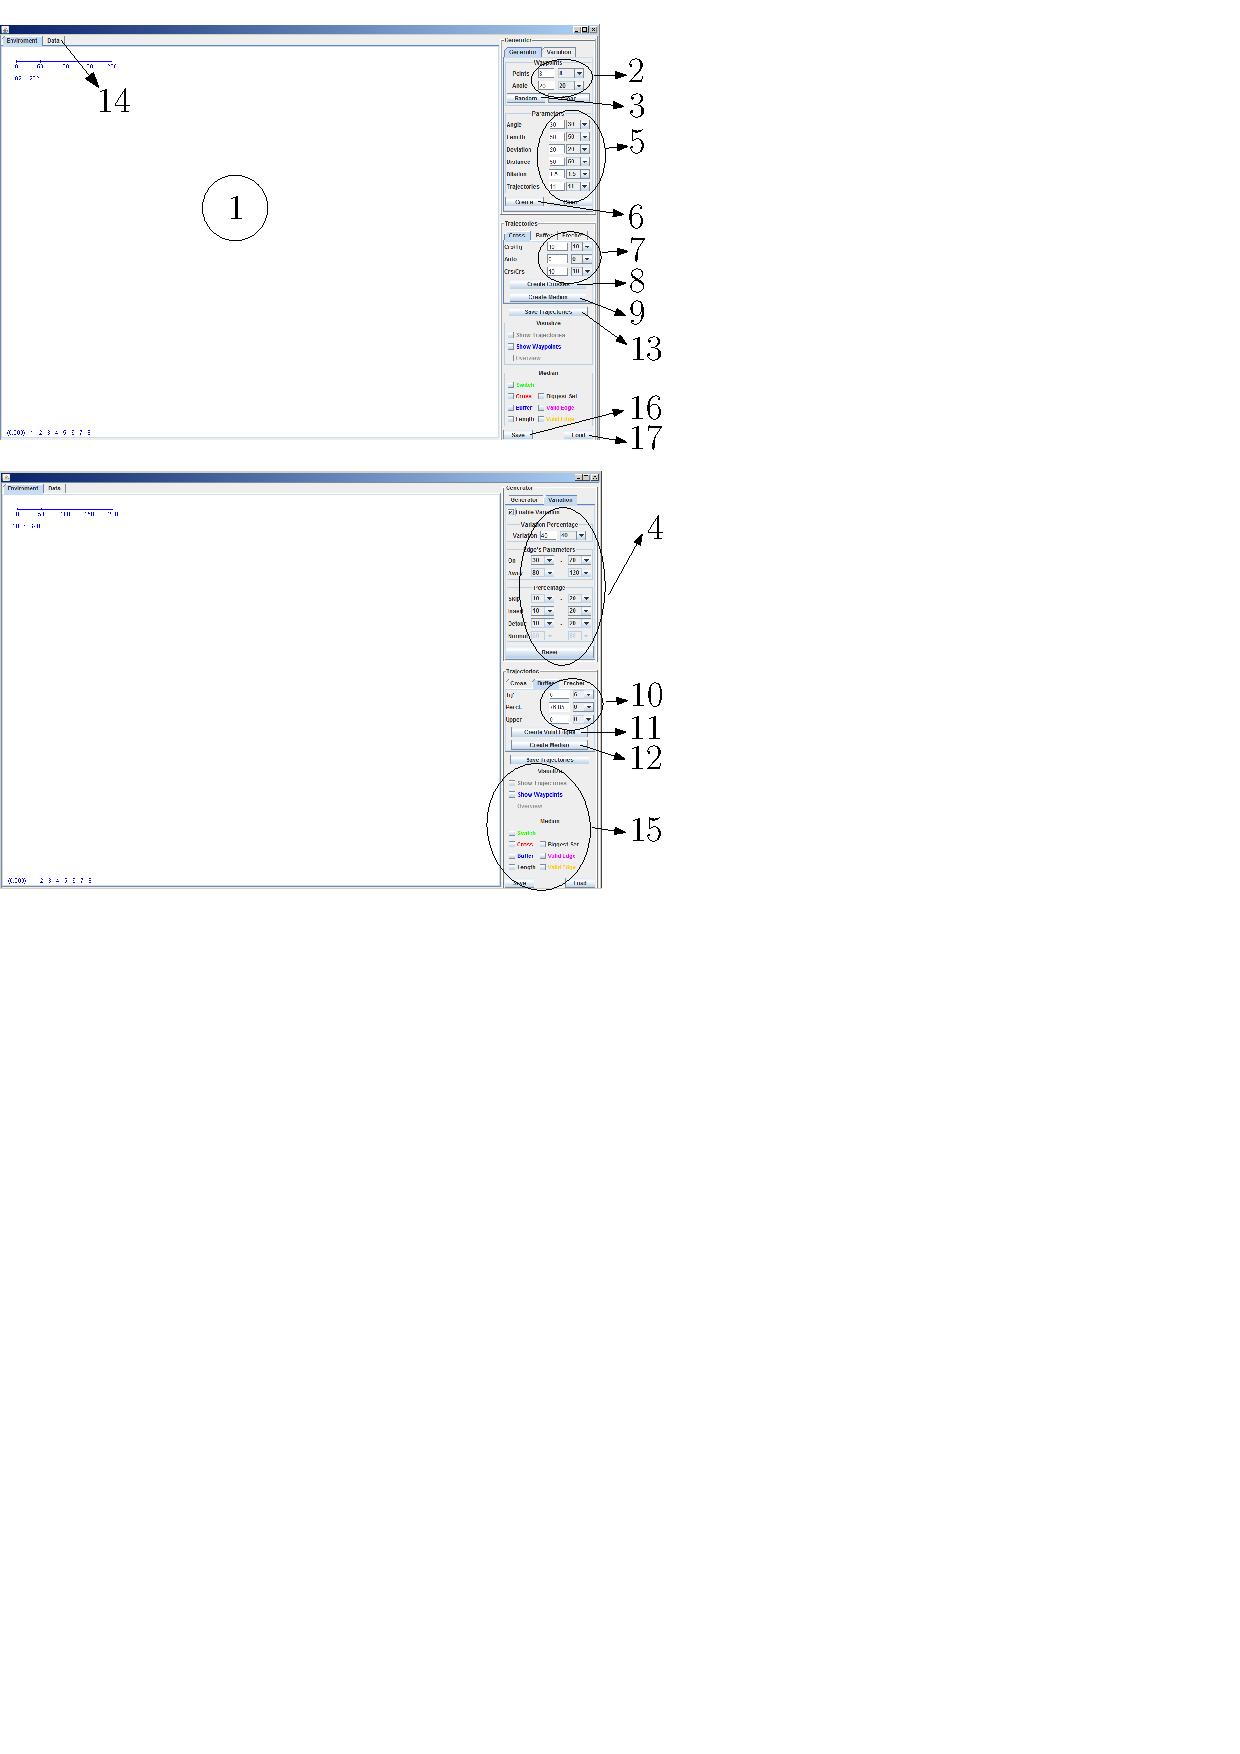
\includegraphics[scale=1]{Gambar/appxa2}
\caption[Interface of the program]{Interface of the program} 
\label{fig:appxa2}
\end{figure}

Step by step to compute the median trajectory using the program:
\begin{enumerate}
\item
Create several waypoints. 
Click anywhere in the ``Environment'' area(1) or create them automatically by setting the parameters for waypoint(2) or clicking the button ``Random''(3).
\item
The ``Variation'' tab could be used to create variations by providing values needed to make them(4).
\item
Create a set of trajectories by setting all parameters(5) and clicking the button ``Create''(6).
\item
Compute the median using the homotopic algorithm: 
\begin{itemize}
\item Define all parameters needed for the homotopic algorithm(7).
\item Create crosses by clicking the ``Create Crosses'' button(8).\item Compute the median by clicking the ``Compute Median'' button(9).
\end{itemize}
\item
Compute the median using the switching method and the buffer algorithm: 
\begin{itemize}
\item Define all parameters needed for the buffer algorithm(10).
\item Create valid edges by clicking the ``Create Valid Edges''button(11). 
\item Compute the median by clicking the ``Compute Median''button(12).
\end{itemize}
\item
Save the resulting median by clicking the ``Save Trajectories'' button(13).
The result is saved in the computer memory and can be seen in ``Data'' tab(14) 
\item 
The set of trajectories and its median trajectories will appear in the ``Environment'' area(1) and the user can change what to display by selecting various choices in ``Visualize'' and ``Median'' area(15).
\item
To save all data to the disk, click the ``Save''(16) button. A file dialog menu will appear.
\item
To load data from the disk, click the ``Load''(17) button.
\end{enumerate}